%!TEX root = ../thesis.tex
%*******************************************************************************
%****************************** Third Chapter **********************************
%*******************************************************************************
\chapter{The Upgraded Detector} \label{Chp:TheUpgradedDetector}

% **************************** Define Graphics Path **************************
\ifpdf
    \graphicspath{{Chapter3/Figs/Raster/}{Chapter3/Figs/PDF/}{Chapter3/Figs/}}
\else
    \graphicspath{{Chapter3/Figs/Vector/}{Chapter3/Figs/}}
\fi

\section{The Upgraded Detector}\label{sec:theUpgradedDetector}
Please note that in the following section of text the term upgraded and VIDARR detector are used interchangeably. The upgraded detector will have 21 more layers than the previous detector going from 49 to 70 layers and the 3 missing columns in side a are also now instrumented. This means the number of channels have increased from 1793 to 2660 which results in an increase of mass by $\sim$ 50\,\%, thus improving the fiducial volume of the detector. This means that more energy from the gadolinium cascade is contained within the detector thus allowing for more effective noise reduction when triggering. Therefore the increase in layers will allow for a higher efficiency of neutron capture. The increase in layers will not yield a significant increase in positron efficiency as positrons are effectively contained to a $\sim$ 99\,\% level with both 1793 channels and 2660 channels as they are contained within 1-2 bars.
\\\\The electronics have also been improved significantly compared to the original detector. The original electronics were carried over from the T2K Ecal, they were the first generation of the technology with relatively high noise rates compared to the current generation used in the VIDARR detector. The energy resolution of the electronics have been greatly increased \hl{(any quantifiable numbers for this stuff?)}. And the noise rates for the original electronics were also more susceptible to changes in temperature than the electronics in the upgraded detector. In addition the upgraded detector will also have field-programmable gate array (FPGA) boards which connect with analogue boards which in turn connect to the MPPCs. The use of FPGA boards allow for more complex trigger functions to be used with up to two thresholds to be used and allows for the summed energy and the number of bars to be hit to be used for trigger discrimination. Which should allow for better signal to noise discrimination than the original detector.
\\\\A basic cut investigation used a form of machine learning called a support vector machine (SVM) to determine the best cut and which dimensions gave the best separation. The cut was dominated by the number of bars hit at the lower threshold of 0.1\,MeV, the most accurate cut would have been utilising the number of bars hit above 0.1\,MeV and the summed energy above the 0.1\,MeV threshold. However due to the structure of the FPGA boards and their programming it was more prudent to use the number of bars hit above both the 0.1\,MeV thresholds and 0.5\,MeV threshold. The cost in classifier accuracy was minimal and it allowed for faster development of the FPGA firmware. 
\\\\To lessen temperature fluctuations in the VIDARR detector the cooling in and around the detector module has been greatly increased from the prototype. The original detector had six radiator fins on 2 sides of the detector which were primarily aimed at cooling the TFBs on each fin. The upgraded VIDARR detector will also have these fins which will help cool the new boards but on the same 2 sides as the fins there will also be two new radiators behind the fins which run the width and height of a side. Greatly increasing the speed that heat will dissipate inside the detector. This will allow for a more consistent temperature  thus reducing dark noise even further from the MPPCs. 

\section{Detector Construction}\label{sec:DetectorConstruction}
The detector construction was a process that was sadly disrupted due to the COVID-19 pandemic which is still on going. The detector construction originally started in November of 2018 with the cutting and painting of scintillation bars that would add the additional mass to the detector. This process was completed by December of 2018. In December of 2018 the original detector was moved out of the shipping container which housed it (figure \ref{fig:detCon000_TakeOut1}). It was then placed inside a clean room opened and disassembled (figure \ref{fig:detCon002_OldTearAway}). The original electronics configuration was not suitable for the upgrade which due to the increased power draw of the new electronics also required a substantial increase in active cooling. Then new scintillator was purchased from Fermi-lab which was $\sim$ twice as long as required. This new scintillator was then cut (figure \ref{subFig:detCon003bb_CuttingScint}) so its dimensions match the old scintillating bars (152\,cm $\times$ 4\,cm $\times$ 1\,cm) and fit exactly inside the detector casing. Once this was done the edges of the freshly cut scintillator were arranged and painted with Ti0$_2$ paint (figure \ref{subFig:detCon005b_PaintingEnds}) to help reflect the light. The cut and painted scintillator was then placed inside the housing for the detector  whilst it was in the clean room (figure \ref{fig:detCon006_RonInCleanRoom}).

\begin{figure}[htbp]
\centering
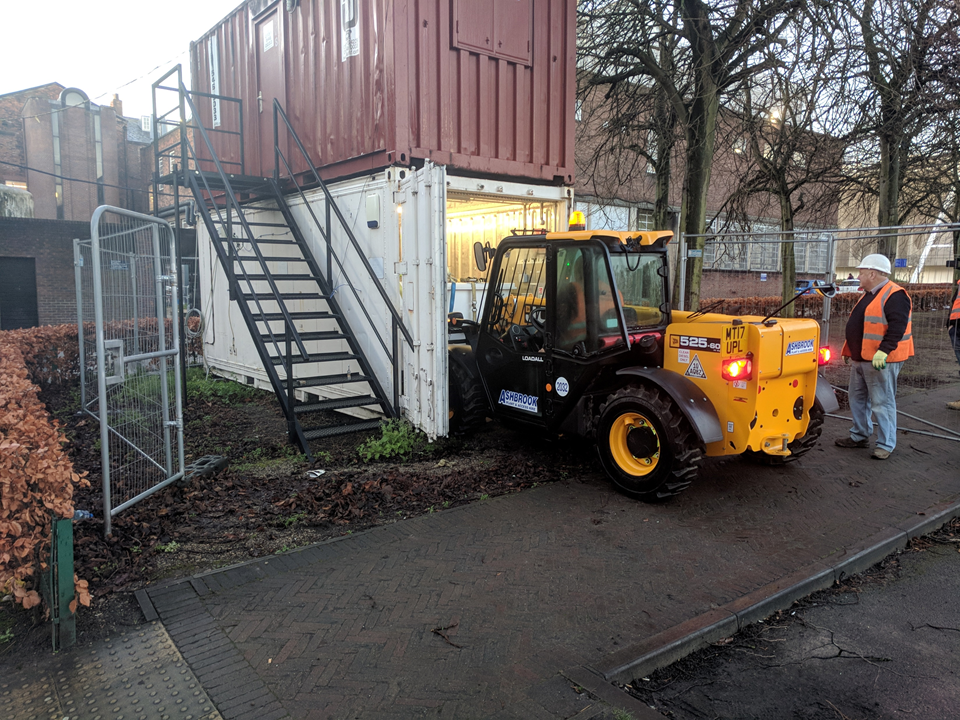
\includegraphics[width=0.8\linewidth]{Chapter3/Figs/Raster/detCon000_TakeOut1.png}
\captionof{figure}{The prototype detector being taken out of the original shipping container which was a standard cool ``meat locker.''} 
\label{fig:detCon000_TakeOut1}
\end{figure}

\begin{figure}[htbp]
\centering
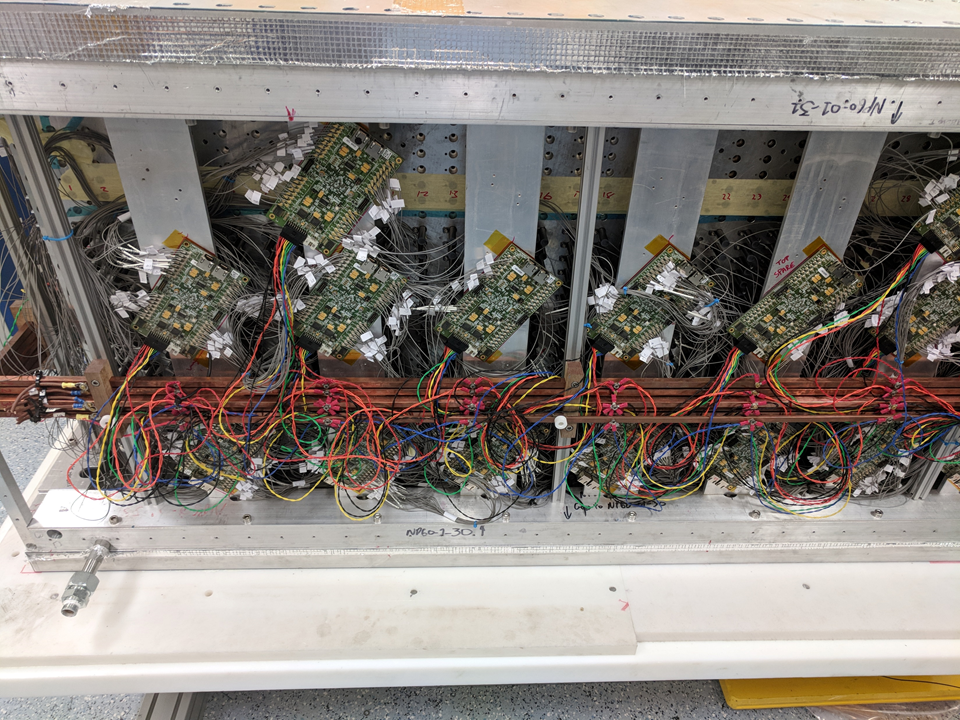
\includegraphics[width=0.8\linewidth]{Chapter3/Figs/Raster/detCon002_OldTearAway.png}
\captionof{figure}{A view of the electronics in the prototype detector. There is much available space in between the boards and the detector itself. The cables are 100\,mm long.} 
\label{fig:detCon002_OldTearAway}
\end{figure}

\begin{figure}[htbp]
\centering
\begin{subfigure}{.5\textwidth}
  \centering
  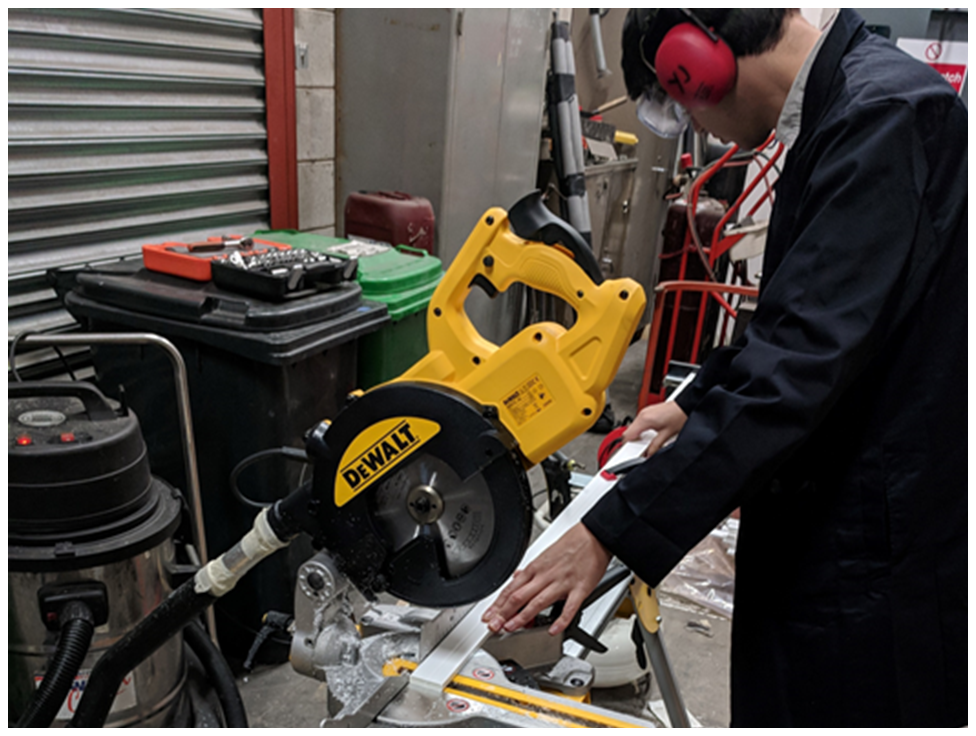
\includegraphics[width=\linewidth]{Chapter3/Figs/Raster/detCon003bb_CuttingScint.png}
  \captionsetup{width=.9\linewidth}
  \caption{Fellow collaborator Yan-Jie Schnellbach cutting scintillator.}
  \label{subFig:detCon003bb_CuttingScint}
\end{subfigure}%
\begin{subfigure}{.5\textwidth}
  \centering
  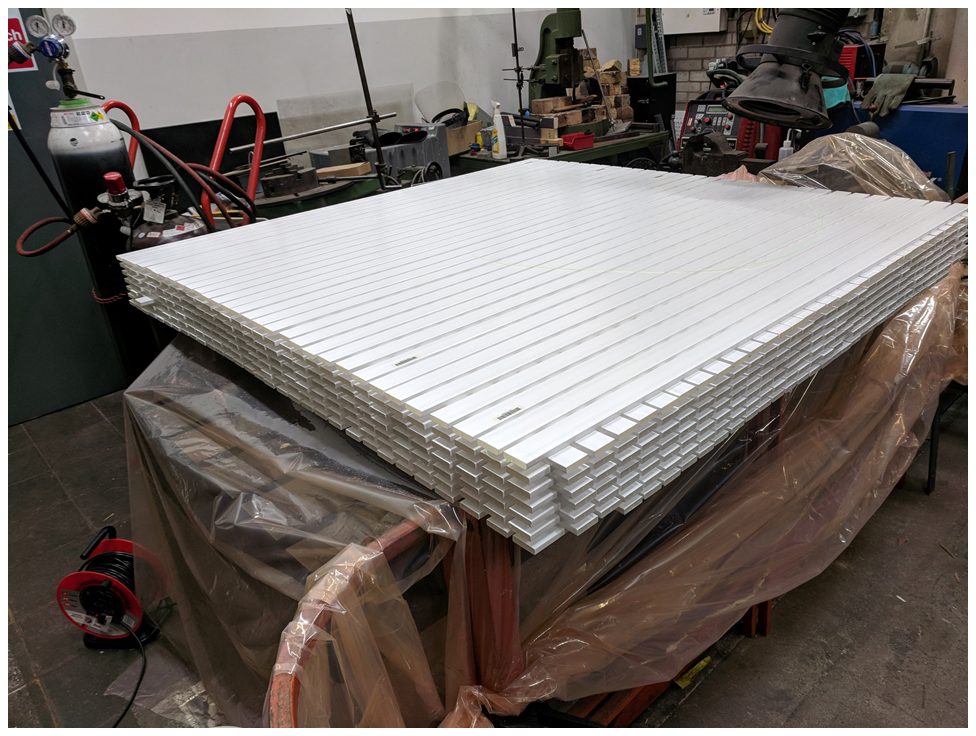
\includegraphics[width=\linewidth]{Chapter3/Figs/Raster/detCon005b_PaintingEnds.png}
  \captionsetup{width=.9\linewidth}
  \caption{The scintillator being arranged for painting the ends of the scintillator.}
  \label{subFig:detCon005b_PaintingEnds}
\end{subfigure}
\caption{Scintillator preparation for being placed inside the detector casing.}
\label{fig:detCon_CuttingScint_PaintingEnds}
\end{figure}

\begin{figure}[htbp]
\centering
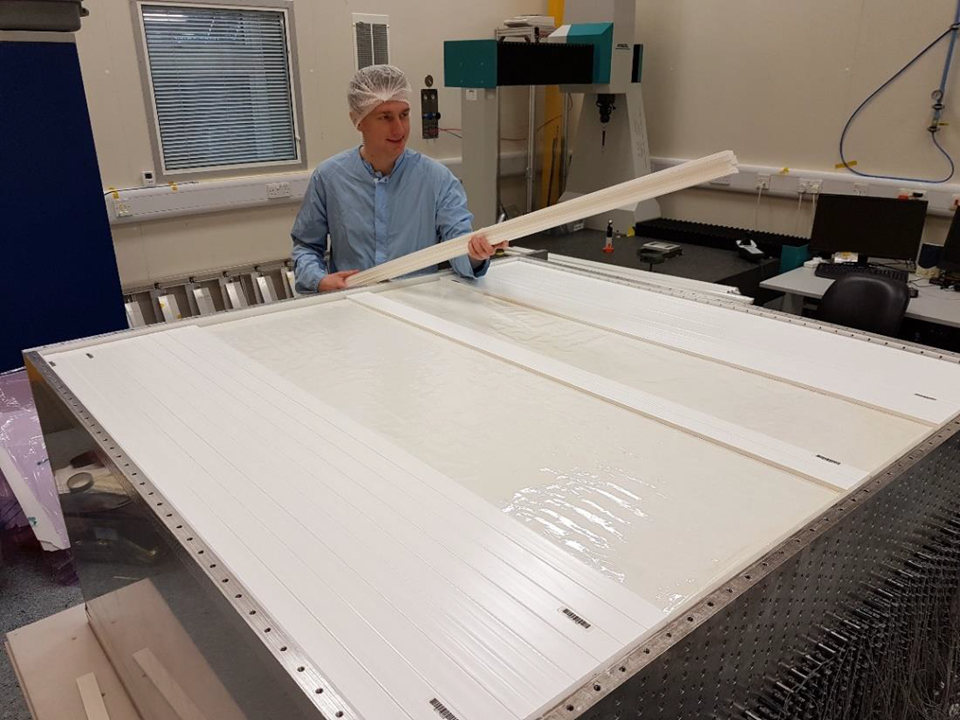
\includegraphics[width=0.8\linewidth]{Chapter3/Figs/Raster/detCon006_RonInCleanRoom.png}
\captionof{figure}{Me (Ronald Collins) in the clean room putting scintillator into the detector. The white sheet of Gadolinium Oxide in-between the layers is also visible.} 
\label{fig:detCon006_RonInCleanRoom}
\end{figure}

One of the major improvements made during the upgrade of the VIDARR detector was an increase in cooling. The original detector had much space between the electronic boards and the MPPCs with the electronic boards placed directly on cooling fins seen in figure \ref{fig:detCon002_OldTearAway}. In addition to the cooling fins seen in figure \ref{fig:detCon002_OldTearAway} large radiators was also added in-between the cooling fins and the MPPCs for each side. These new radiators are comprised of large stainless steel plates which was cut using a water cutter shown in figure \ref{subFig:detCon011b_RadiatorConstruction}. Then copper piping was placed through the sections seen in figure \ref{subFig:detCon012b_RadiatorPiping}. This copper piping will face the MPPCs and detector scintillator whilst the radiator fins will be attached behind the radiator away from the MPPCs and behind insulation. As in the prototype the electronic boards will be placed on the fins similar to figure \ref{fig:detCon002_OldTearAway}. This should improve the cooling in the detector significantly as the heat from the electronic boards should be isolated from scintillator and the MPPCs when compared to the prototype. 

\begin{figure}[htbp]
\centering
\begin{subfigure}{.5\textwidth}
  \centering
  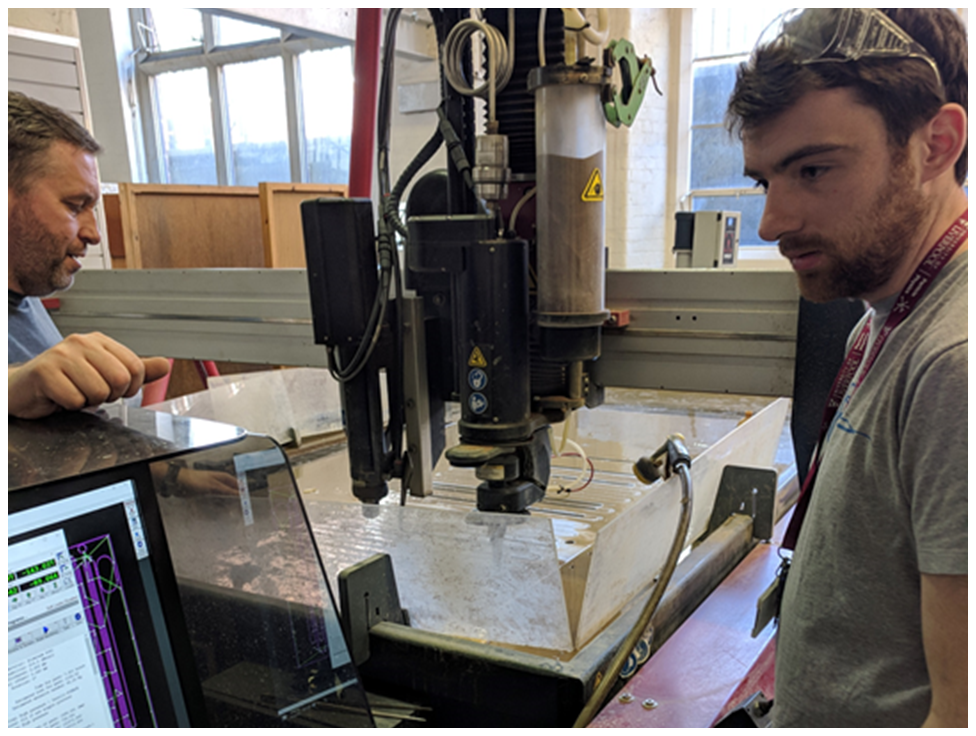
\includegraphics[width=\linewidth]{Chapter3/Figs/Raster/detCon011b_RadiatorConstruction.png}
  \captionsetup{width=.9\linewidth}
  \caption{The steel frame of the new radiator being cut .}
  \label{subFig:detCon011b_RadiatorConstruction}
\end{subfigure}%
\begin{subfigure}{.5\textwidth}
  \centering
  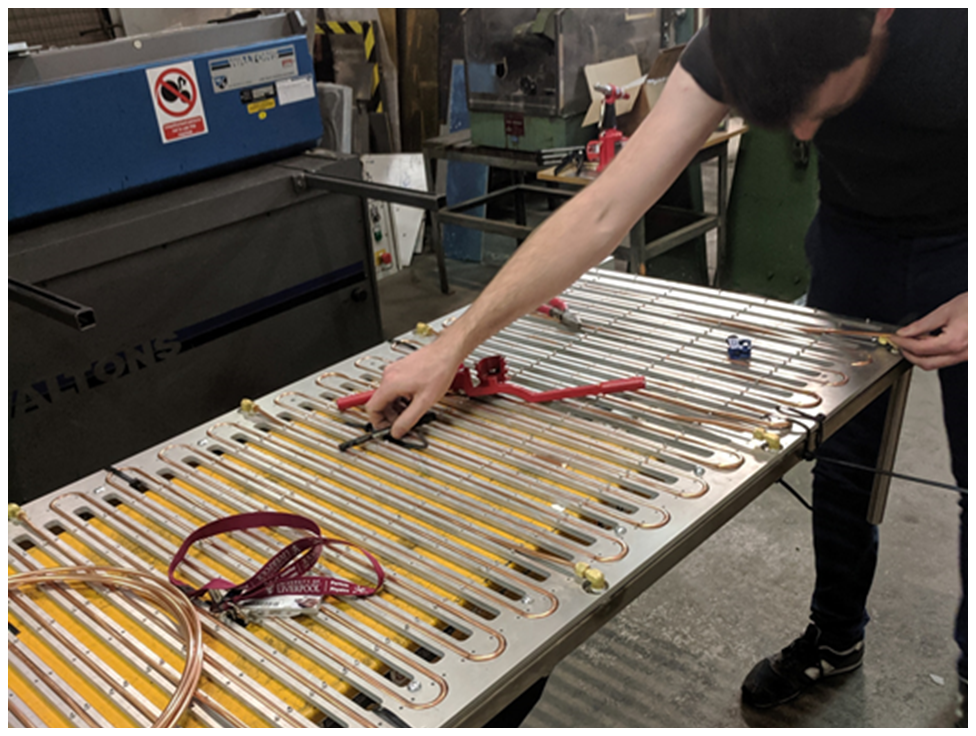
\includegraphics[width=\linewidth]{Chapter3/Figs/Raster/detCon012b_RadiatorPiping.png}
  \captionsetup{width=.9\linewidth}
  \caption{The new radiator having the piping inserted.}
  \label{subFig:detCon012b_RadiatorPiping}
\end{subfigure}
\caption{The construction of the new radiator which has more active cooling and larger surface area than the original radiator. \hl{numbers for cooling anywhere?}}
\label{fig:detCon_RadiatorConstruction_RadiatorPiping}
\end{figure}

Once the scintillator is in the detector casing several individual components need to be assembled so that the light emitted by the scintillator can then be analysed. The light emitted by the scintillator is first picked up by the Wavelength shifting (WLS) fibres. These fibres are threaded through the centre of the scintillator and capture light and shift it to green light seen in figure \ref{subFig:detCon013b_WlsFibres}. These WLS fibres then have 3d printed connectors glued on to the ends of them as seen in figure \ref{subFig:detCon014b_WlsWithEnds}. Then the holders for the MPPCs which attach to the connectors on the WLS fibres need to be 3D printed seen in figure \ref{fig:detCon_3dPrintedHolders_3dPrintedFreed} both with and without supporting struts (figures \ref{subFig:detCon015b_3dPrintedHolders} \ref{subFig:detCon016b_3dPrintedFreed} respectively). Then PCBs which connect the MPPCs to the coaxial cables need to be produced a sheet of which can be seen in figure \ref{subFig:detCon008b_PlacingPcbs}. These PCBs have to have a coaxial cable connector soldered on to them and pins pushed through them so they can pick up the signals that the MPPCs produce. A finished example of one of these PCBs can be seen in figure \ref{subFig:detCon009b_SoloPcb}. The holders PCBs and MPPCs all fit together as shown in figure \ref{fig:detCon017b_HoldersWithParts}.

\begin{figure}[htbp]
\centering
\begin{subfigure}{.5\textwidth}
  \centering
  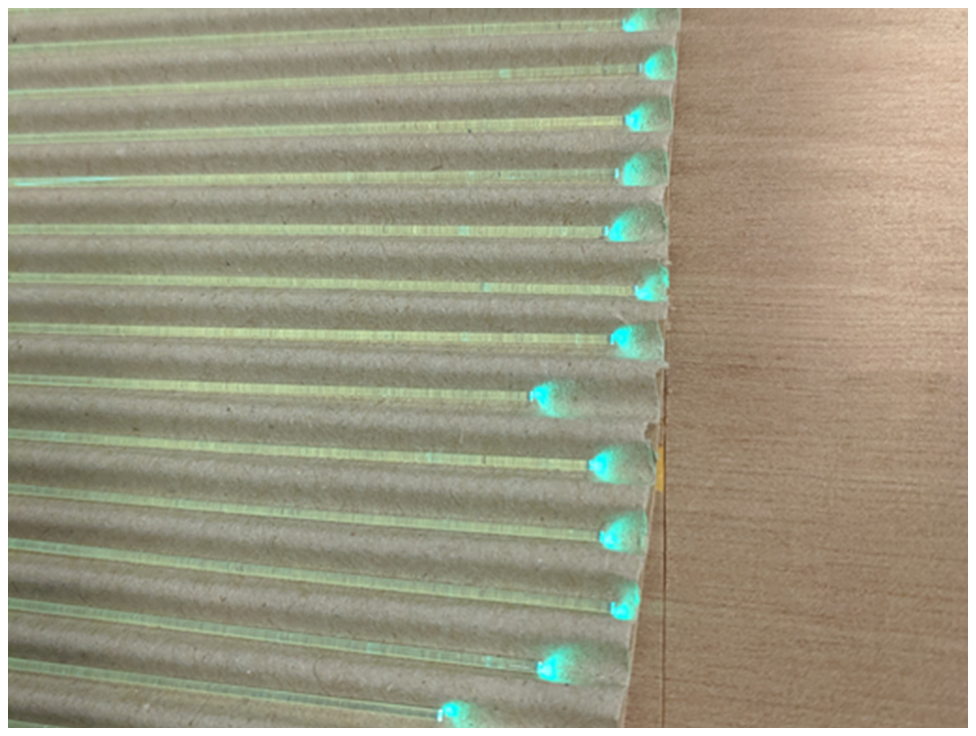
\includegraphics[width=\linewidth]{Chapter3/Figs/Raster/detCon013b_WlsFibres.png}
  \captionsetup{width=.9\linewidth}
  \caption{The WLS fibres which are threaded into the scintillator.}
  \label{subFig:detCon013b_WlsFibres}
\end{subfigure}%
\begin{subfigure}{.5\textwidth}
  \centering
  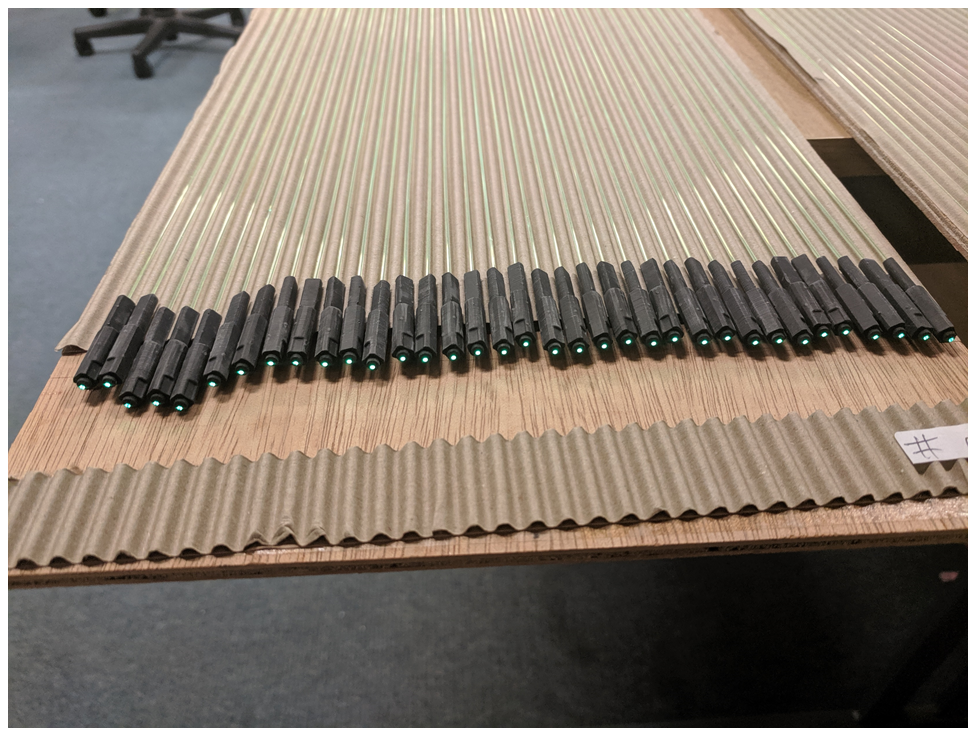
\includegraphics[width=\linewidth]{Chapter3/Figs/Raster/detCon014b_WlsWithEnds.png}
  \captionsetup{width=.9\linewidth}
  \caption{The WLS fibres with ends which connect to the plastic holders which house the MPPCs.}
  \label{subFig:detCon014b_WlsWithEnds}
\end{subfigure}
\caption{The WLS fibres which will funnel light from the scintillator to the MPPCs. They are assembled on cardboard and have 3d printed ends glued onto them.}
\label{fig:detCon_WlsFibres_WlsWithEnds}
\end{figure}

\begin{figure}[htbp]
\centering
\begin{subfigure}{.5\textwidth}
  \centering
  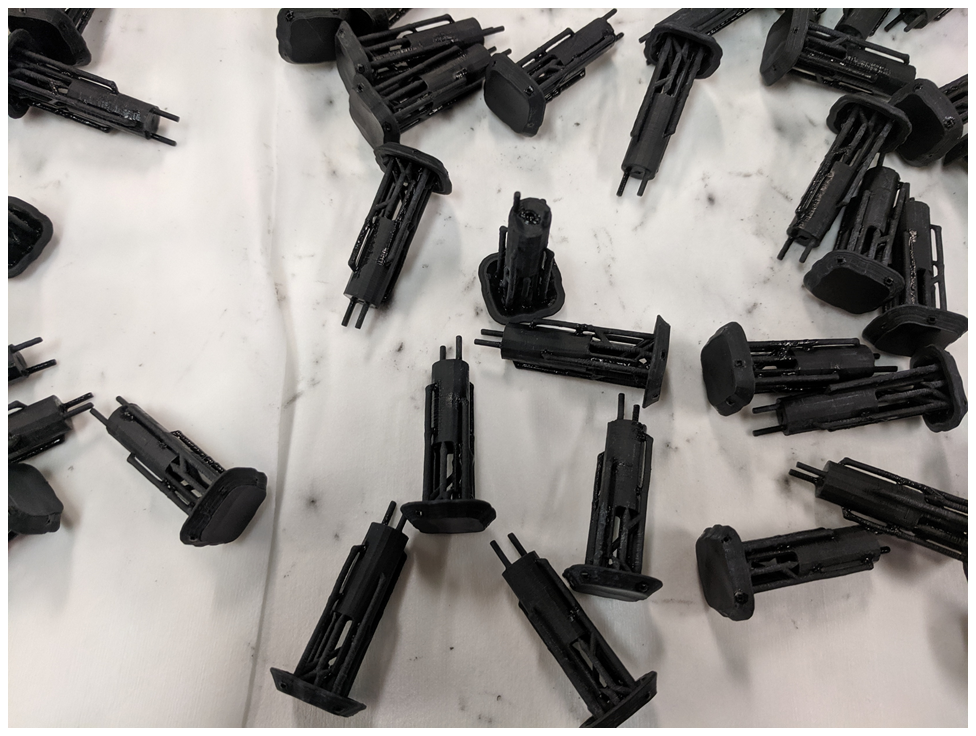
\includegraphics[width=\linewidth]{Chapter3/Figs/Raster/detCon015b_3dPrintedHolders.png}
  \captionsetup{width=.9\linewidth}
  \caption{3D printed holders for the MPPCs and PCBs with supporting struts.}
  \label{subFig:detCon015b_3dPrintedHolders}
\end{subfigure}%
\begin{subfigure}{.5\textwidth}
  \centering
  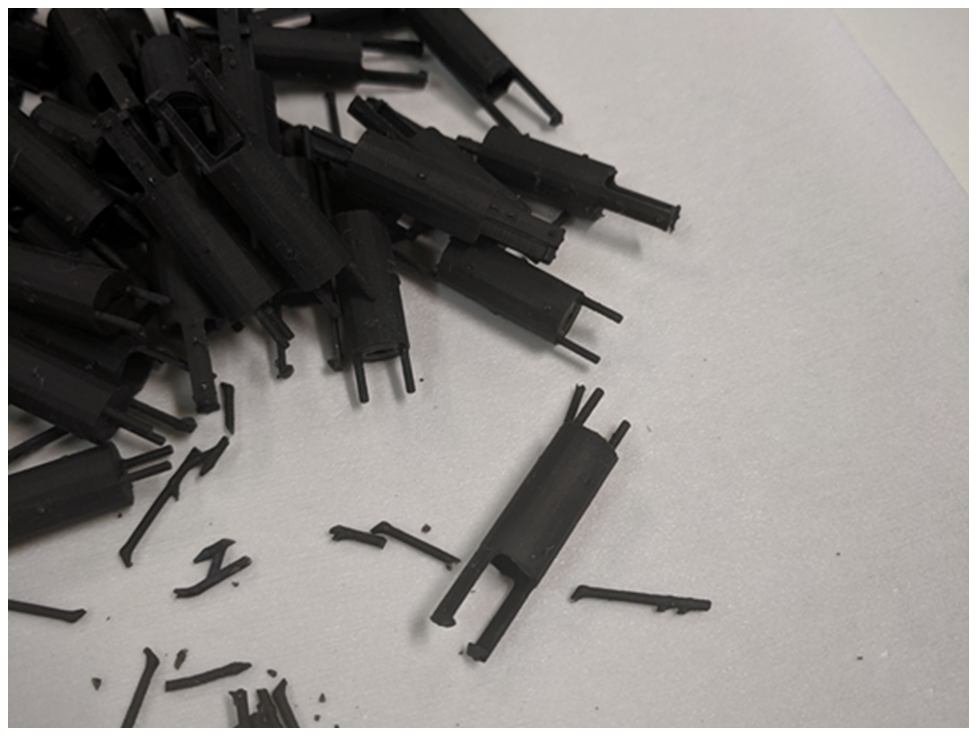
\includegraphics[width=\linewidth]{Chapter3/Figs/Raster/detCon016b_3dPrintedFreed.png}
  \captionsetup{width=.9\linewidth}
  \caption{3D printed holders for the MPPCs and PCBs freed from their struts .}
  \label{subFig:detCon016b_3dPrintedFreed}
\end{subfigure}
\caption{The holders for the MPPCs and the PCBs. Holders for the additional channels needed to be 3D printed as more from the original supply chain could not be procured. }
\label{fig:detCon_3dPrintedHolders_3dPrintedFreed}
\end{figure}

\begin{figure}[htbp]
\centering
\begin{subfigure}{.5\textwidth}
  \centering
  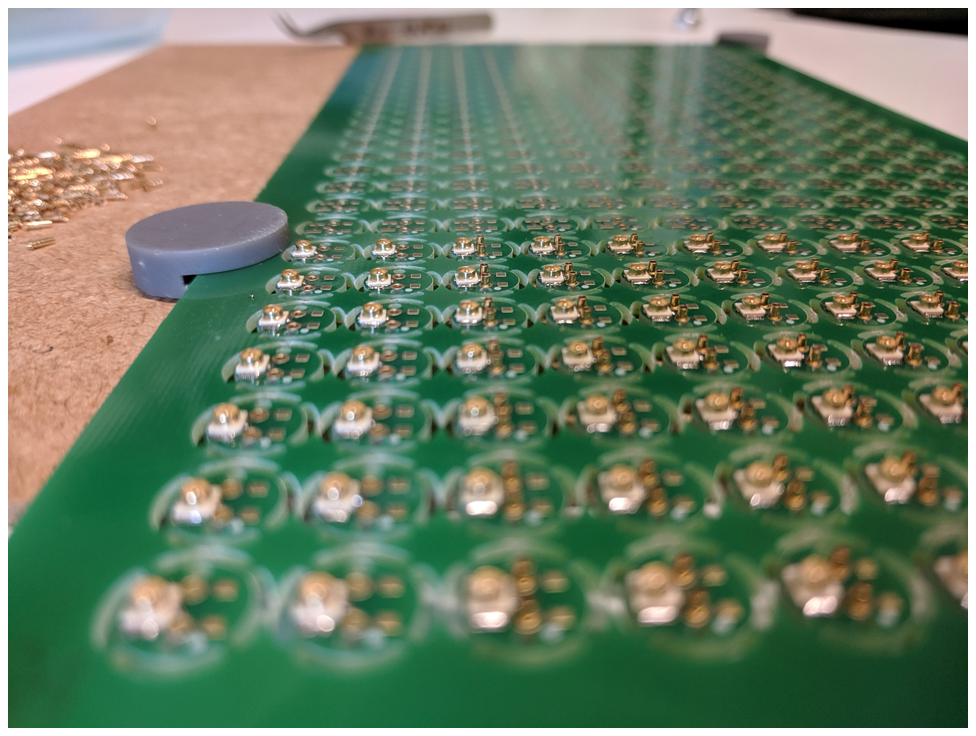
\includegraphics[width=\linewidth]{Chapter3/Figs/Raster/detCon008b_PlacingPcbs.png}
  \captionsetup{width=.9\linewidth}
  \caption{A sheet of PCB boards being assembled. Slightly elevated for putting in  pins.}
  \label{subFig:detCon008b_PlacingPcbs}
\end{subfigure}%
\begin{subfigure}{.5\textwidth}
  \centering
  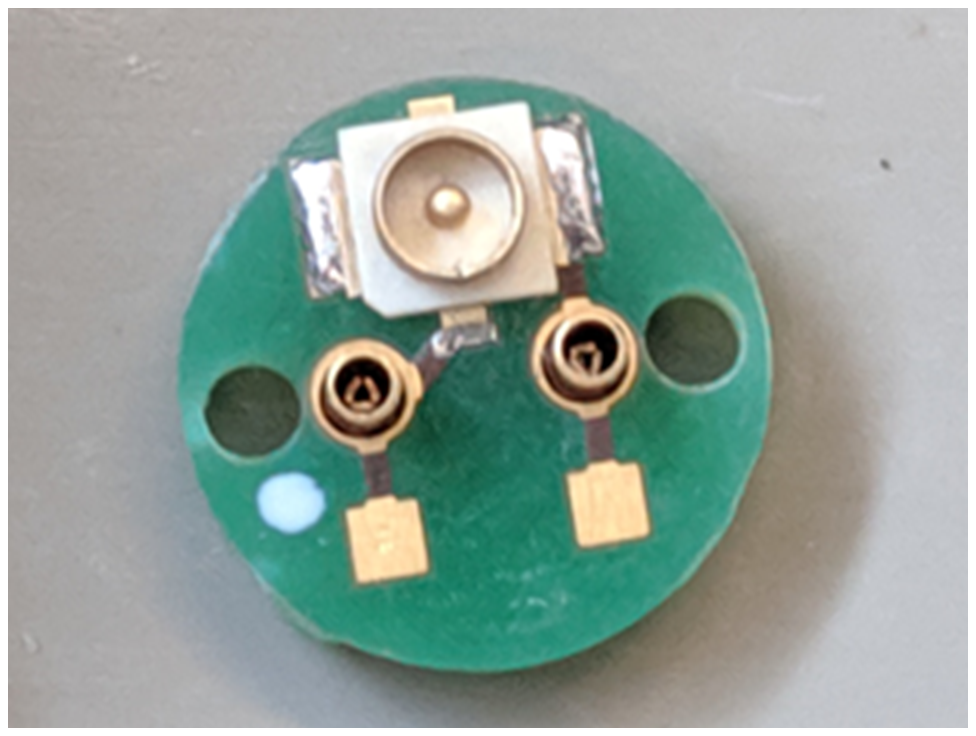
\includegraphics[width=\linewidth]{Chapter3/Figs/Raster/detCon009b_SoloPcb.png}
  \captionsetup{width=.9\linewidth}
  \caption{A finished solo PCB that connects to the MPPC.}
  \label{subFig:detCon009b_SoloPcb}
\end{subfigure}
\caption{The assembly of the PCBs which attach to the MPPCs through pins. The connector at the top of the PCBs is where the cables are attached.}
\label{fig:detCon_PlacingPcbs_SoloPcb}
\end{figure}

\begin{figure}[htbp]
\centering
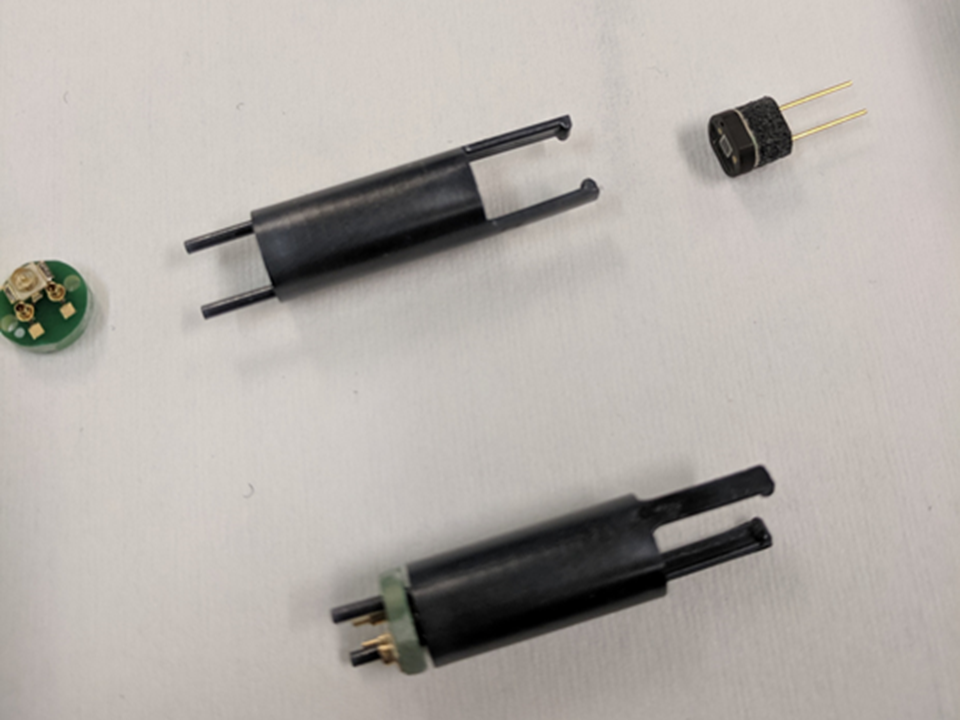
\includegraphics[width=0.8\linewidth]{Chapter3/Figs/Raster/detCon017b_HoldersWithParts.png}
\captionof{figure}{Holder next to MPPC and PCB (Top) and holder with assembled components (Bottom). Note the the MPPC in the top right is actually reversed from its correct orientation, the prongs of the MPPC go through the PCB board pins.} 
\label{fig:detCon017b_HoldersWithParts}
\end{figure}

Once the components for measuring the light from the WLS fibres were assembled the coaxial cables needed labels. The labels are printed out by the machine seen in figure  \ref{subFig:detCon018b_HeatLabelsPrinted}. This machine prints the labels in long streams which then need to be cut into individual labels seen in figure \ref{subFig:detCon019b_CutLabels}. These labels are in the form side-row-column with the bottom left of each side being the coordinate for (0,0). These labels are then slid onto the coaxial cables at 8\,cm from the end of the side that connects to the boards as seen in figure \ref{subFig:detCon020b_LabelsLoose}. A heat gun is used to shrink the lbels onto the coaxial cables as seen in figure \ref{subFig:detCon021b_LabelsHeated}. These cables are then connected to the holders as seen in figure \ref{fig:detCon023b_HoldersConnectedZoom} where the PCB connector seen in figure \ref{subFig:detCon009b_SoloPcb} connects firmly to the cable. The holder is also put into a sheath so that it is held firmly in place once inside the detector.

\begin{figure}[htbp]
\centering
\begin{subfigure}{.5\textwidth}
  \centering
  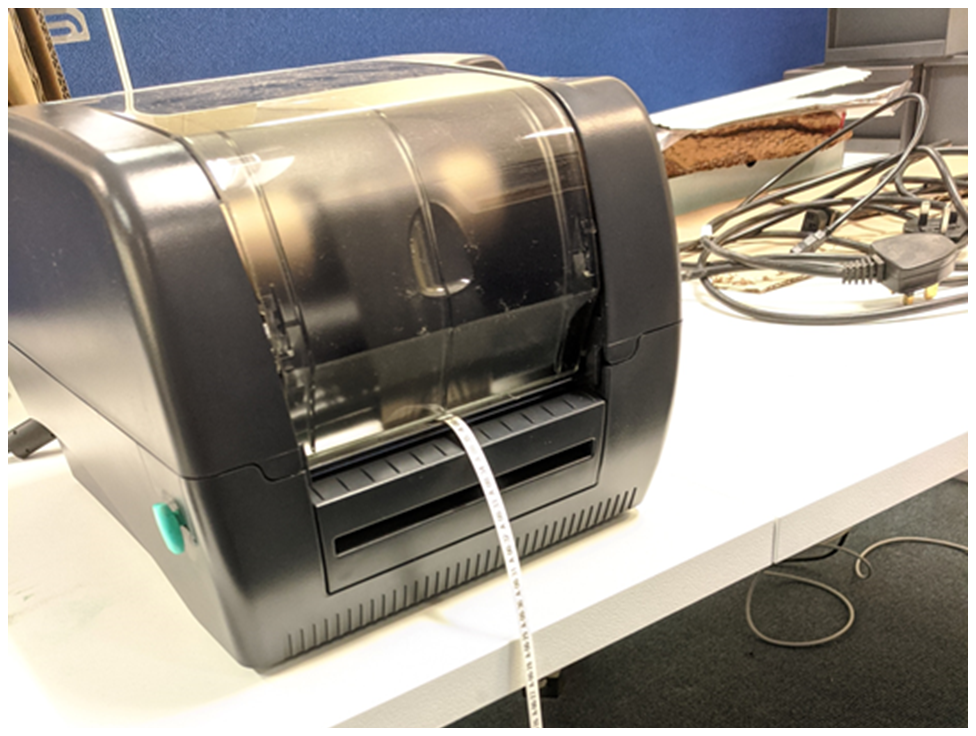
\includegraphics[width=\linewidth]{Chapter3/Figs/Raster/detCon018b_HeatLabelsPrinted.png}
  \captionsetup{width=.9\linewidth}
  \caption{Heat shrink labels being printed out.}
  \label{subFig:detCon018b_HeatLabelsPrinted}
\end{subfigure}%
\begin{subfigure}{.5\textwidth}
  \centering
  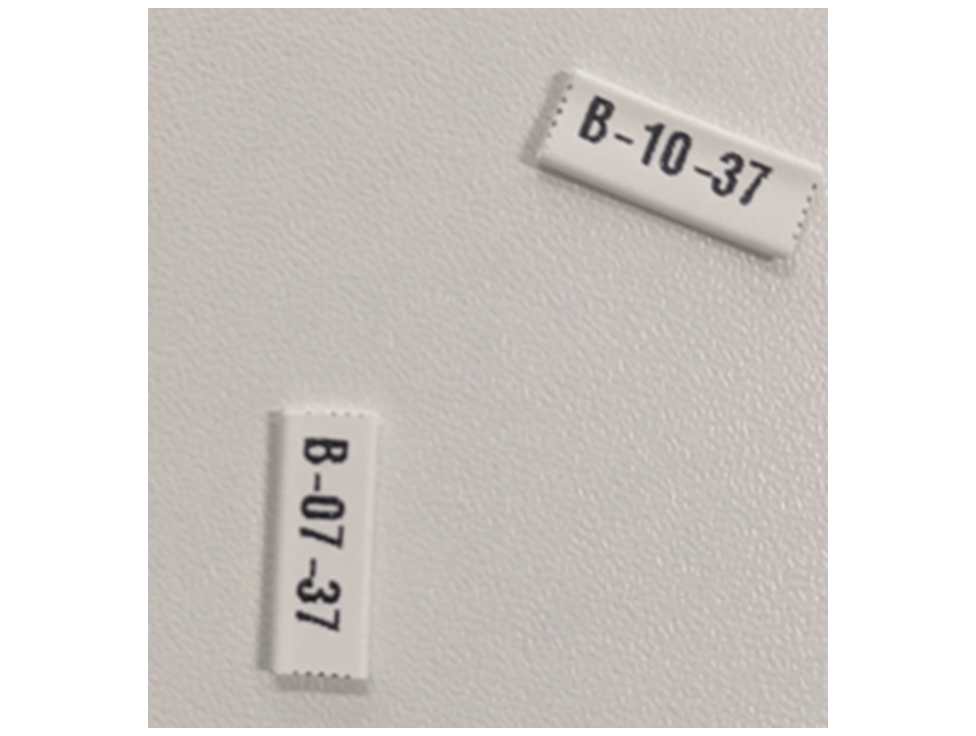
\includegraphics[width=\linewidth]{Chapter3/Figs/Raster/detCon019b_CutLabels.png}
  \captionsetup{width=.9\linewidth}
  \caption{Individual labels for specific cables.}
  \label{subFig:detCon019b_CutLabels}
\end{subfigure}
\caption{Heat shrink labels that are used to identify cables. Labels are printed out in the form side-Row-Column where bottom left is (0,0) }
\label{fig:detCon_HeatLabelsPrinted_CutLabels}
\end{figure}

\begin{figure}[htbp]
\centering
\begin{subfigure}{.5\textwidth}
  \centering
  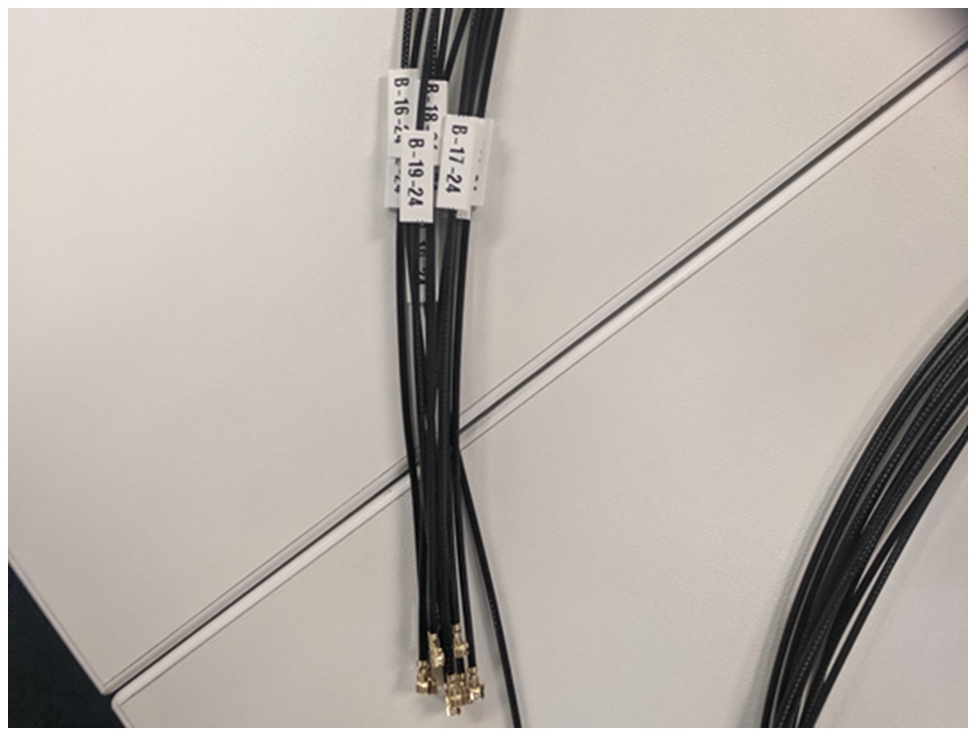
\includegraphics[width=\linewidth]{Chapter3/Figs/Raster/detCon020b_LabelsLoose.png}
  \captionsetup{width=.9\linewidth}
  \caption{Labels threaded onto the cables loosely .}
  \label{subFig:detCon020b_LabelsLoose}
\end{subfigure}%
\begin{subfigure}{.5\textwidth}
  \centering
  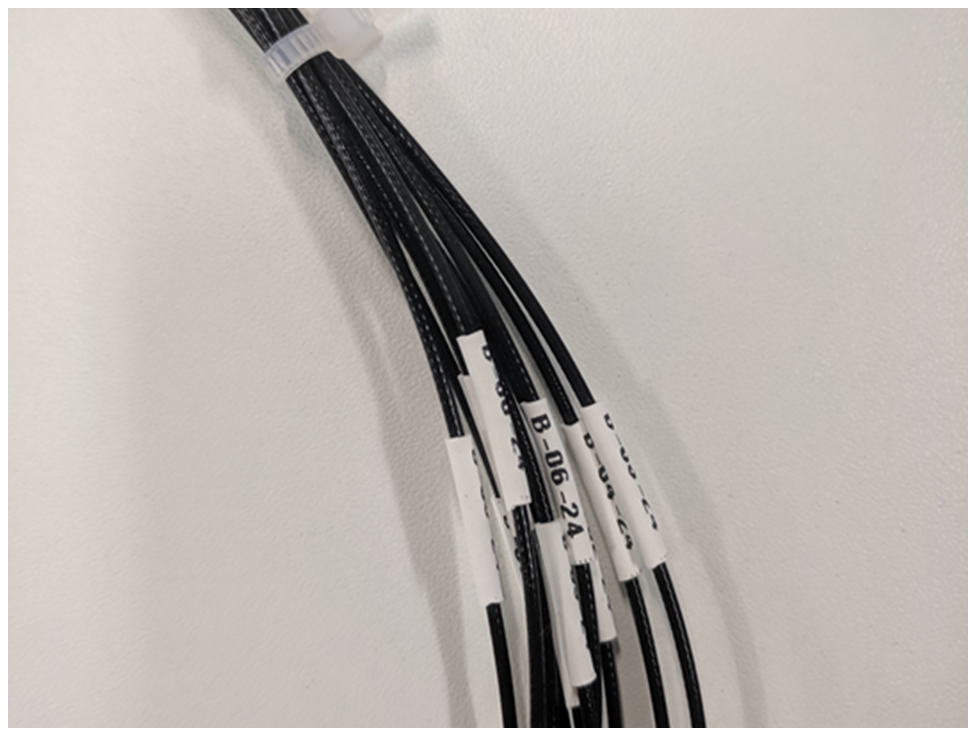
\includegraphics[width=\linewidth]{Chapter3/Figs/Raster/detCon021b_LabelsHeated.png}
  \captionsetup{width=.9\linewidth}
  \caption{The heated labels have shrunk.}
  \label{subFig:detCon021b_LabelsHeated}
\end{subfigure}
\caption{Labels are threaded through at 8\,cm from the end of the cables as seen in \ref{subFig:detCon020b_LabelsLoose} then a heat gun is used on the cables to shrink the labels and they are bunched as seen in in \ref{subFig:detCon021b_LabelsHeated}.}
\label{fig:detCon_LabelsLoose_LabelsHeated}
\end{figure}

\begin{figure}[htbp]
\centering
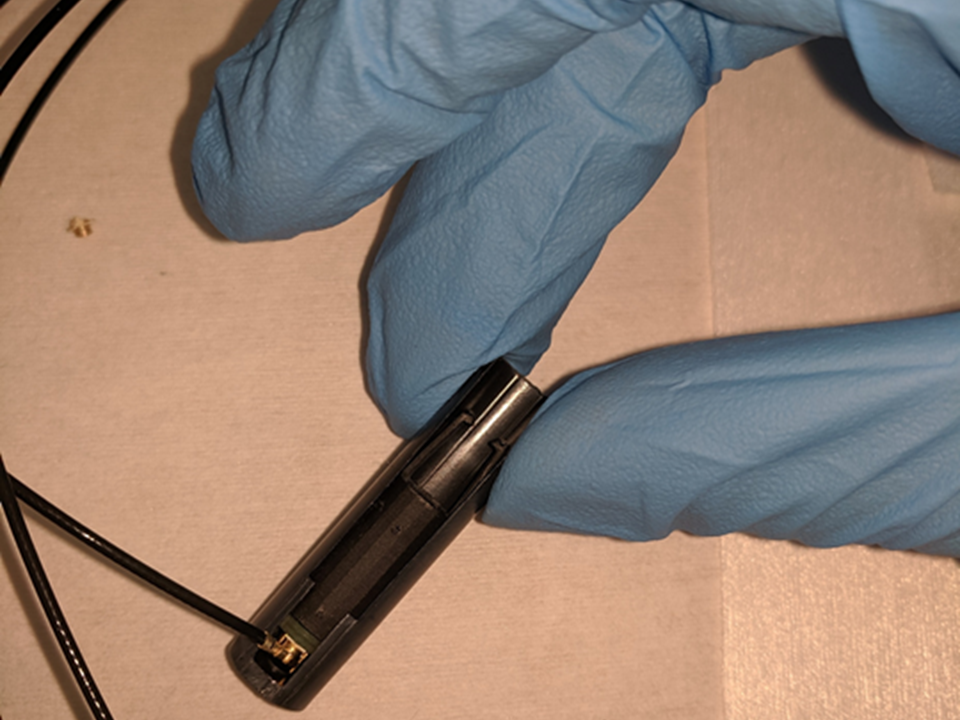
\includegraphics[width=0.8\linewidth]{Chapter3/Figs/Raster/detCon023b_HoldersConnectedZoom.png}
\captionof{figure}{The holder connected to a cable and put inside a sheath.} 
\label{fig:detCon023b_HoldersConnectedZoom}
\end{figure}

All of the MPPC holders in their sheaths with connected cables are then connected to the WLS fibres and their connectors shown in figure \ref{subFig:detCon014b_WlsWithEnds}. There are two distinct sheath types the grey which are made via injection moulding and orange sheaths which were 3d printed. These sheaths protect the rest of the components and can be seen clearly in figure \ref{fig:detCon_HaningOffRadiator_RadiatorTopDown} as they protrude from the detector casing. The radiator was slowly moved into position as cables were thread through the insulation as can be seen in figure \ref{subFig:detCon026b_HaningOffRadiator}. Once the radiator was moved into position the space between the radiator and sheaths was checked to ensure that no undue pressure was being applied to the sheaths which as figure \ref{subFig:detCon028b_RadiatorTopDown} shows there wasn't. Once the radiator was in position the cooling fins were also attached as seen in figure \ref{fig:detCon030b_RadiatorWithFins}. Also in figure \ref{fig:detCon030b_RadiatorWithFins} the x shaped analogue board holders have also been attached with thermal paste to the cooling fins. An example of how the analogue boards are attached to the cooling fins can be seen in figure \ref{fig:detCon032_ConnectedBoard}. Which shows how the cables are connected to the analogue boards and aligned through a cable comb. 

\begin{figure}[htbp]
\centering
\begin{subfigure}{.5\textwidth}
  \centering
  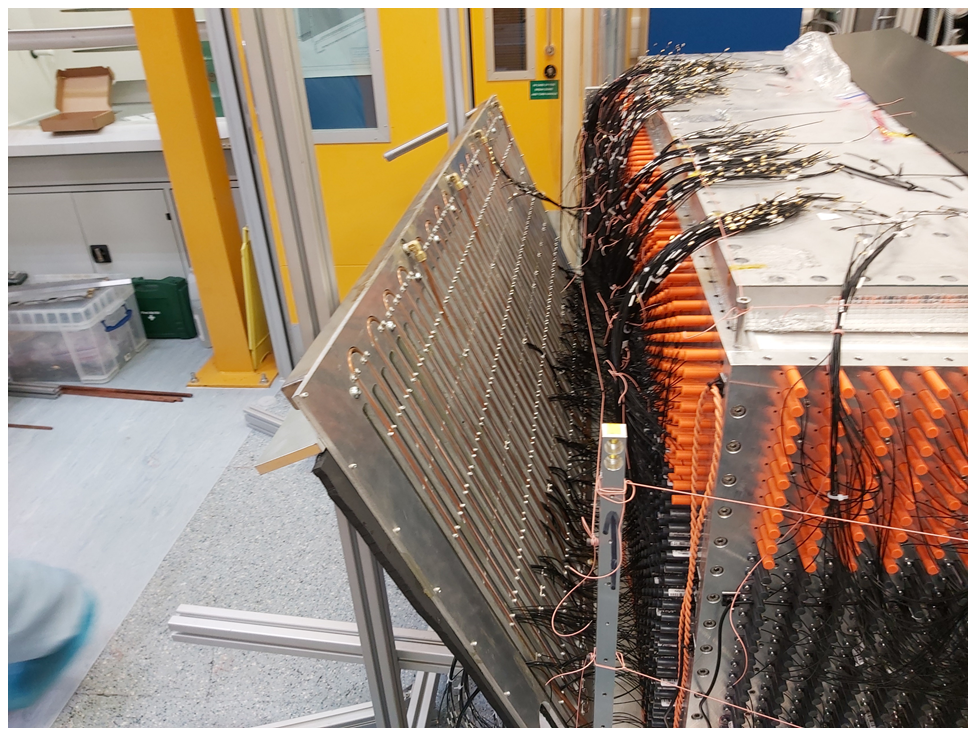
\includegraphics[width=\linewidth]{Chapter3/Figs/Raster/detCon026b_HaningOffRadiator.png}
  \captionsetup{width=.9\linewidth}
  \caption{The side A radiator being positioned into place as cables are placed through the insulation on the radiator.}
  \label{subFig:detCon026b_HaningOffRadiator}
\end{subfigure}%
\begin{subfigure}{.5\textwidth}
  \centering
  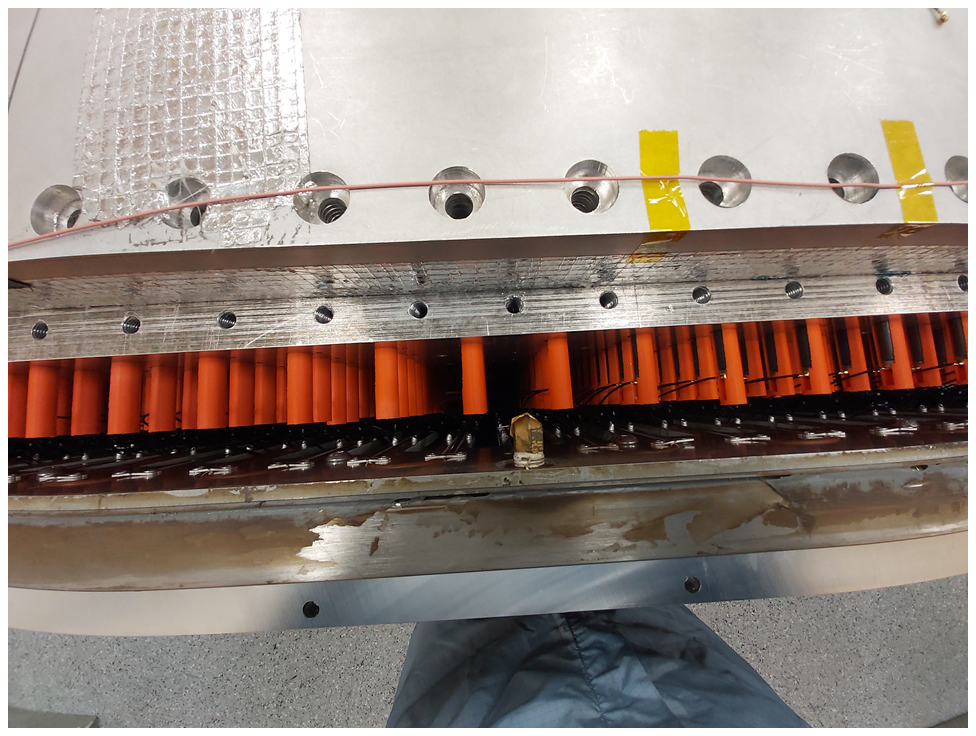
\includegraphics[width=\linewidth]{Chapter3/Figs/Raster/detCon028b_RadiatorTopDown.png}
  \captionsetup{width=.9\linewidth}
  \caption{The side A radiator in position with all of the cables threaded through the insulation. This is minimal space}
  \label{subFig:detCon028b_RadiatorTopDown}
\end{subfigure}
\caption{As part of the upgrade the radiators are significantly larger and do not leave much space between the detector and the electronics.}
\label{fig:detCon_HaningOffRadiator_RadiatorTopDown}
\end{figure}

% \begin{figure}[htbp]
% \centering
% \begin{subfigure}{.5\textwidth}
%   \centering
%   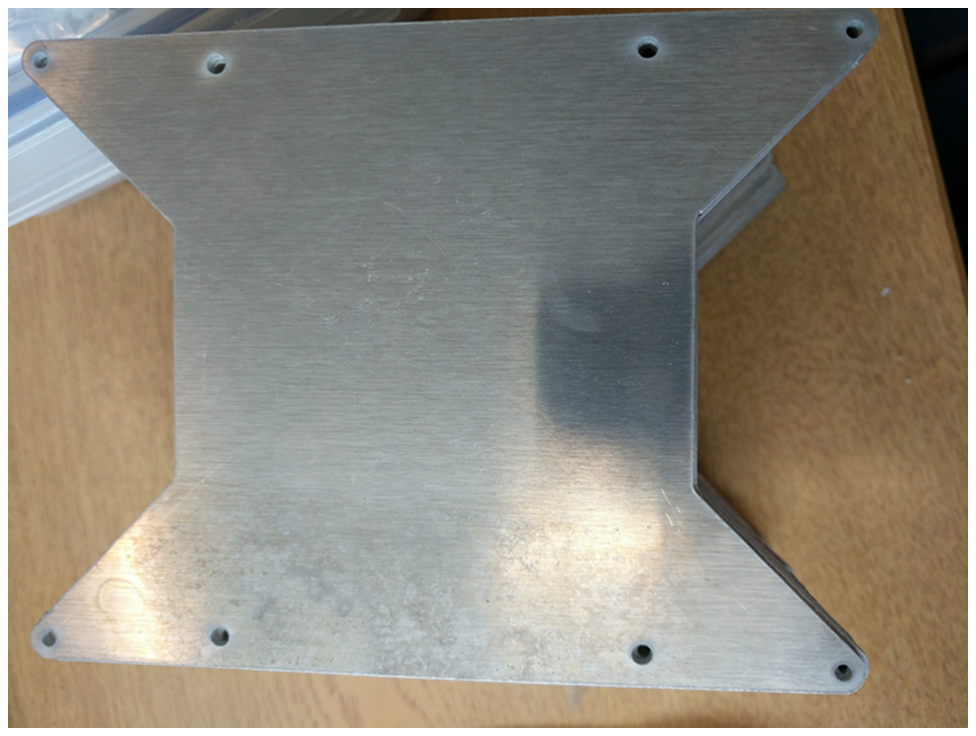
\includegraphics[width=\linewidth]{Chapter3/Figs/Raster/detCon029b_coolantFin.png}
%   \captionsetup{width=.9\linewidth}
%   \caption{Board holders that connect the analogue boards to the cooling fins.}
%   \label{subFig:detCon029b_coolantFin}
% \end{subfigure}%
% \begin{subfigure}{.5\textwidth}
%   \centering
%   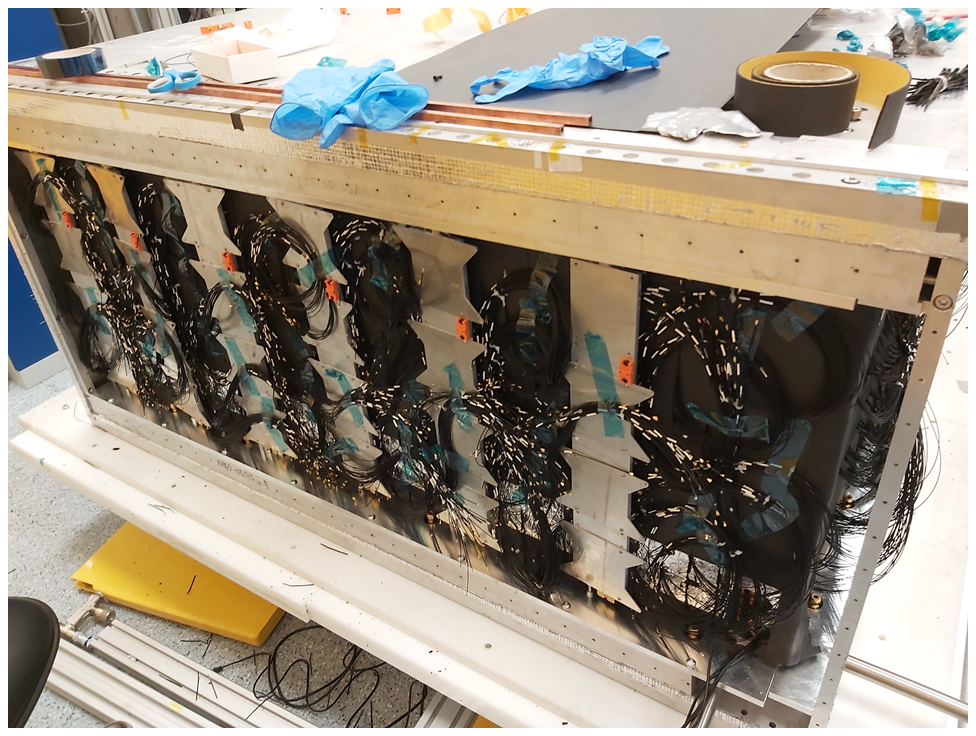
\includegraphics[width=\linewidth]{Chapter3/Figs/Raster/detCon030b_RadiatorWithFins.png}
%   \captionsetup{width=.9\linewidth}
%   \caption{Cooling fins and board holders attached to the radiator.}
%   \label{subFig:detCon030b_RadiatorWithFins}
% \end{subfigure}
% \caption{The analogue board holders and cooling fins are attached after the cables are threaded through the radiator insulation.}
% \label{fig:detCon_coolantFin_RadiatorWithFins}
% \end{figure}

\begin{figure}[htbp]
\centering
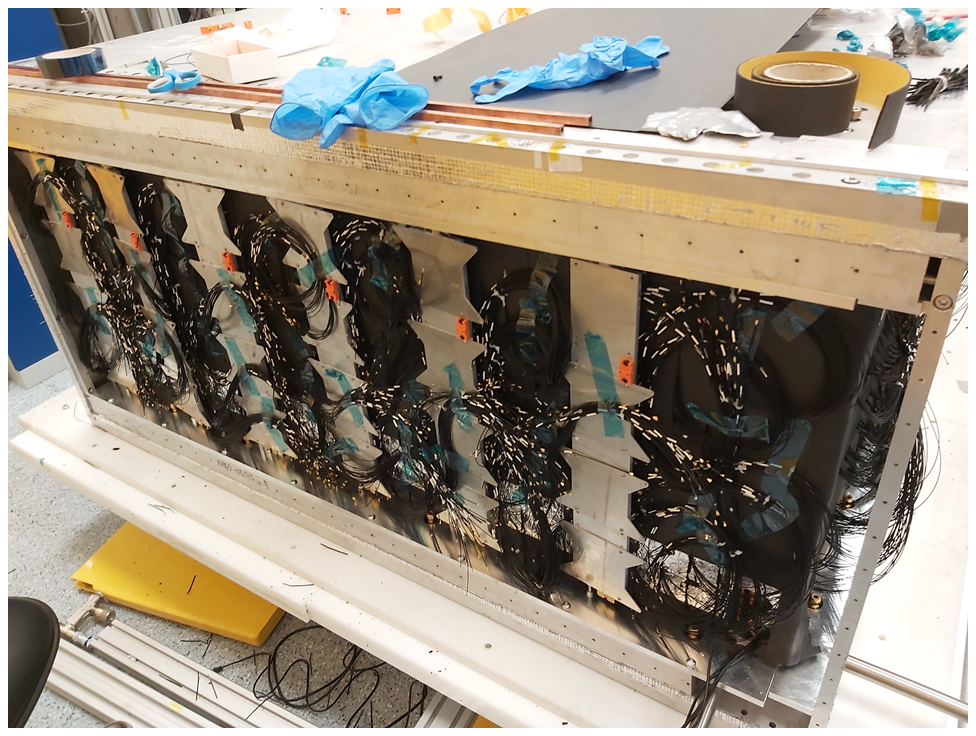
\includegraphics[width=0.8\linewidth]{Chapter3/Figs/Raster/detCon030b_RadiatorWithFins.png}
\captionof{figure}{The radiator on side A with the cooling fins and analogue board holders attached with cables pushed through the insulation and bunched.} 
\label{fig:detCon030b_RadiatorWithFins}
\end{figure}

\begin{figure}[htbp]
\centering
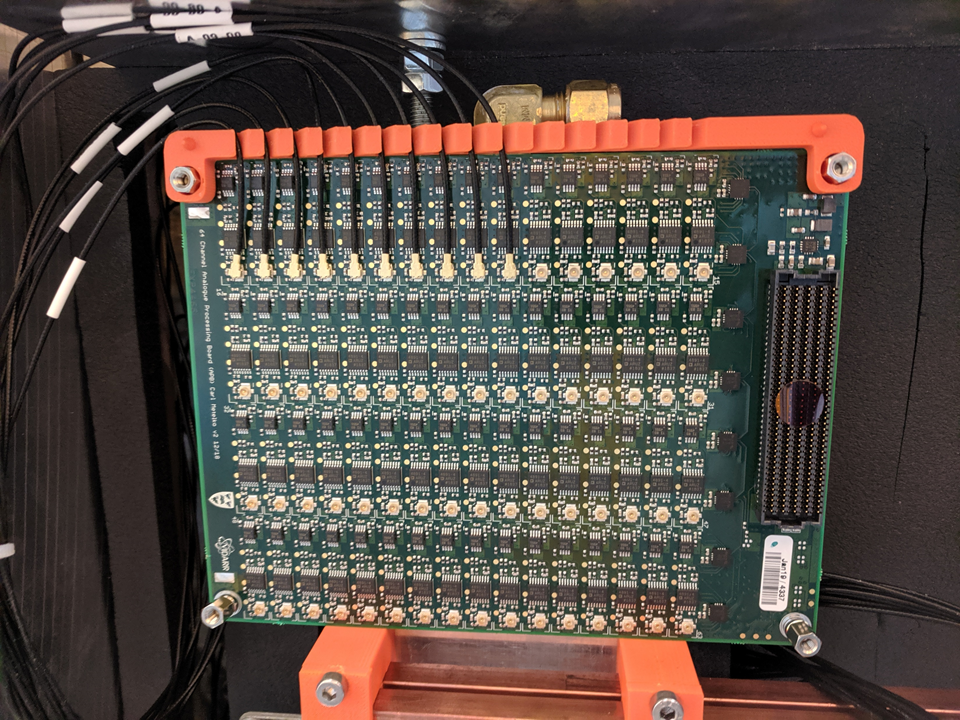
\includegraphics[width=0.8\linewidth]{Chapter3/Figs/Raster/detCon032_ConnectedBoard.png}
\captionof{figure}{An analogue board with some of the cables connected to it. A 3D printed cable ``comb'' is used to align the cables.} 
\label{fig:detCon032_ConnectedBoard}
\end{figure}

The upgraded container was delivered 18$^{th}$ of September 2019 which can be seen \ref{subFig:detCon037c_ContainerArrives}. But it wasn't until 24$^{th}$ of November 2020 that the detector was placed inside its new container (figure \ref{subFig:detCon039b_PutIn2}). The detector upgrade was not complete at this point and currently remains incomplete this is largely due to the COVID-19 pandemic. The upgrade's progressed ceased around the same time as the container arrived during September of 2019 as an issue with electronics was discovered. which currently remains unresolved. Due to the issues in the electronics supply chain caused by the COVID-19 crisis and the small size of the VIDARR collaboration obtaining replacement electronics has been impossible up to September of 2021. Though in recent months there has been some movement in obtaining the relevant components. 

\begin{figure}[htbp]
\centering
\begin{subfigure}{.5\textwidth}
  \centering
  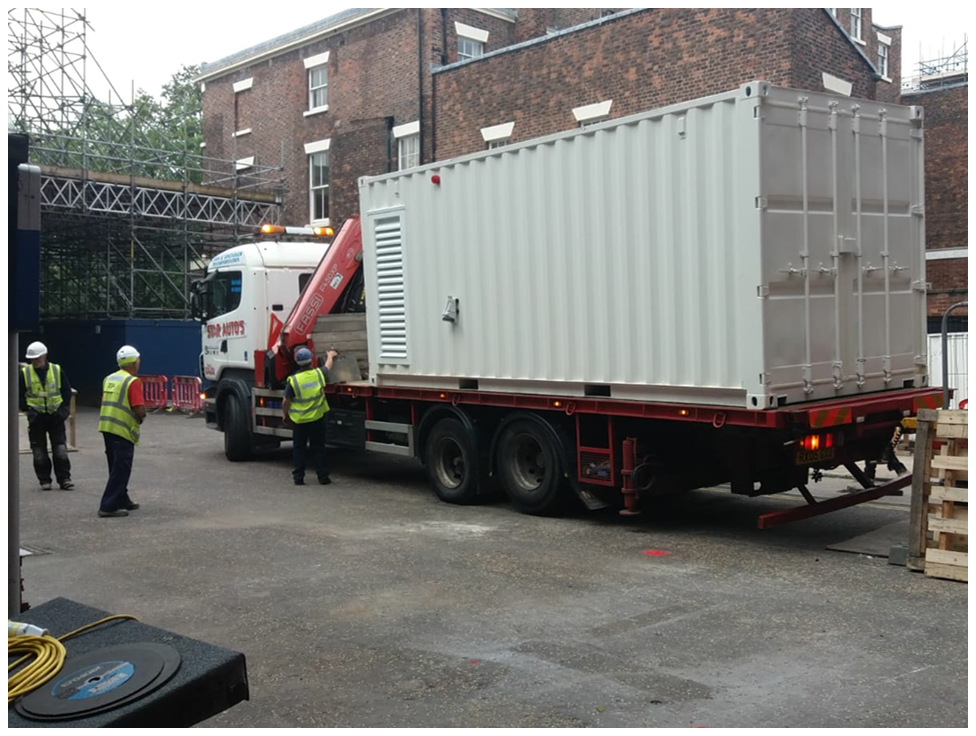
\includegraphics[width=\linewidth]{Chapter3/Figs/Raster/detCon037c_ContainerArrives.png}
  \captionsetup{width=.9\linewidth}
  \caption{The new container arrives at the University of Liverpool.}
  \label{subFig:detCon037c_ContainerArrives}
\end{subfigure}%
\begin{subfigure}{.5\textwidth}
  \centering
  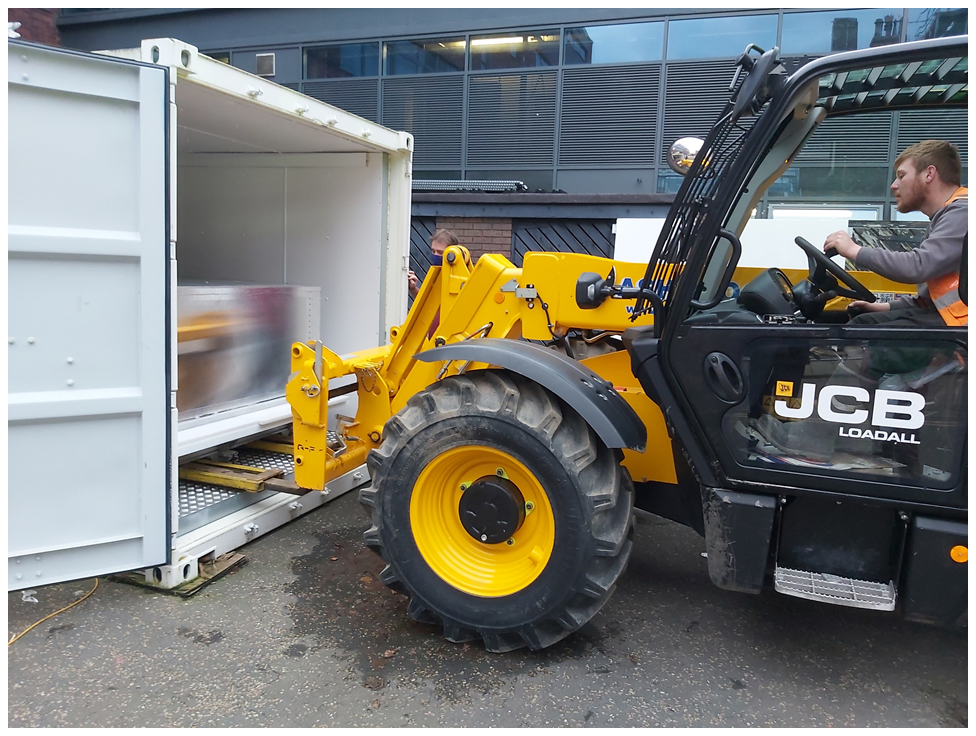
\includegraphics[width=\linewidth]{Chapter3/Figs/Raster/detCon039b_PutIn2.png}
  \captionsetup{width=.9\linewidth}
  \caption{The partially upgraded detector deposited in the new container.}
  \label{subFig:detCon039b_PutIn2}
\end{subfigure}
\caption{The new container arrives and the partially upgraded detector is deposited inside of it.}
\label{fig:detCon_ContainerArrives_PutIn}
\end{figure}

The upgraded container has much improved air flow when compared to the original in figure  \ref{fig:detCon035b_ContainerAirCon} the air conditioning and improved ventilation system can be seen. The upgraded container should be able to keep temperature consistent and thus reduce uncertainties caused by temperature fluctuations. In addition there has been a significant improvement to computational power with both a new computer rack seen in figure \ref{fig:detCon042b_Rack1}. And a powerful new computer with 64 total threads and 64\,Gb of RAM seen in figure \ref{fig:detCon044_NewComputer}. Neither of these are currently in the container due to the issues with COVID-19 previously discussed as they are being used to diagnose any issues with the electronics and analyse older data sets.  

\begin{figure}[htbp]
\centering
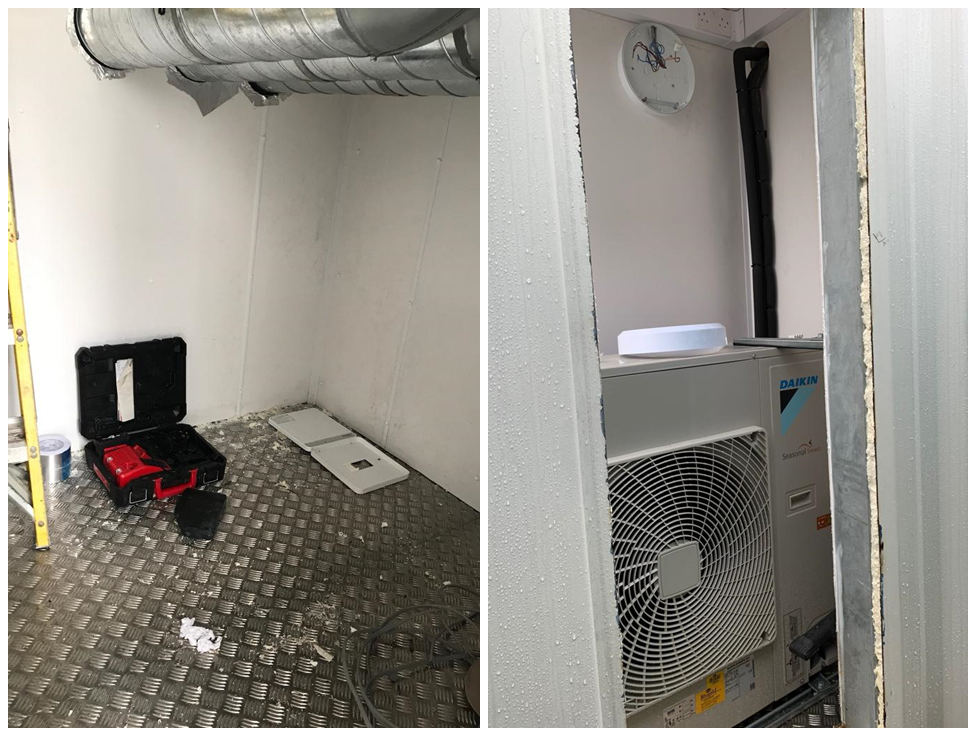
\includegraphics[width=0.7\linewidth]{Chapter3/Figs/Raster/detCon035b_ContainerAirCon.png}
\captionof{figure}{The new container which has an air conditioning and air circulatory system to help keep consistent temperature.} 
\label{fig:detCon035b_ContainerAirCon}
\end{figure}

% \begin{figure}[htbp]
% \centering
% 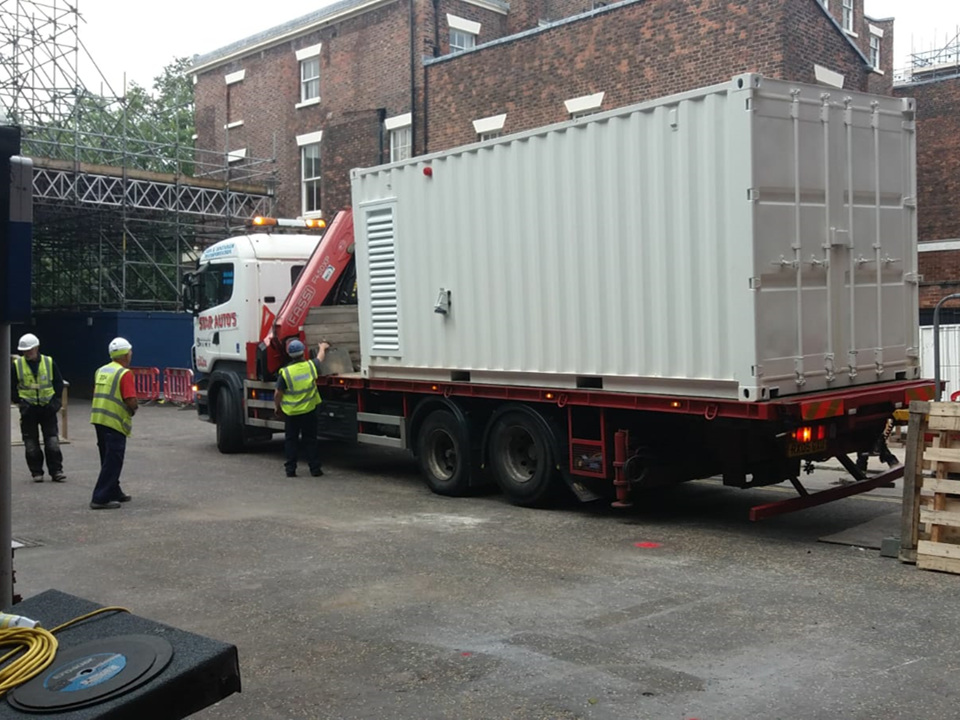
\includegraphics[width=0.8\linewidth]{Chapter3/Figs/Raster/detCon037b_ContainerArrives.png}
% \captionof{figure}{The new container arrives at the University of Liverpool.} 
% \label{fig:detCon037b_ContainerArrives}
% \end{figure}

% \begin{figure}[htbp]
% \centering
% 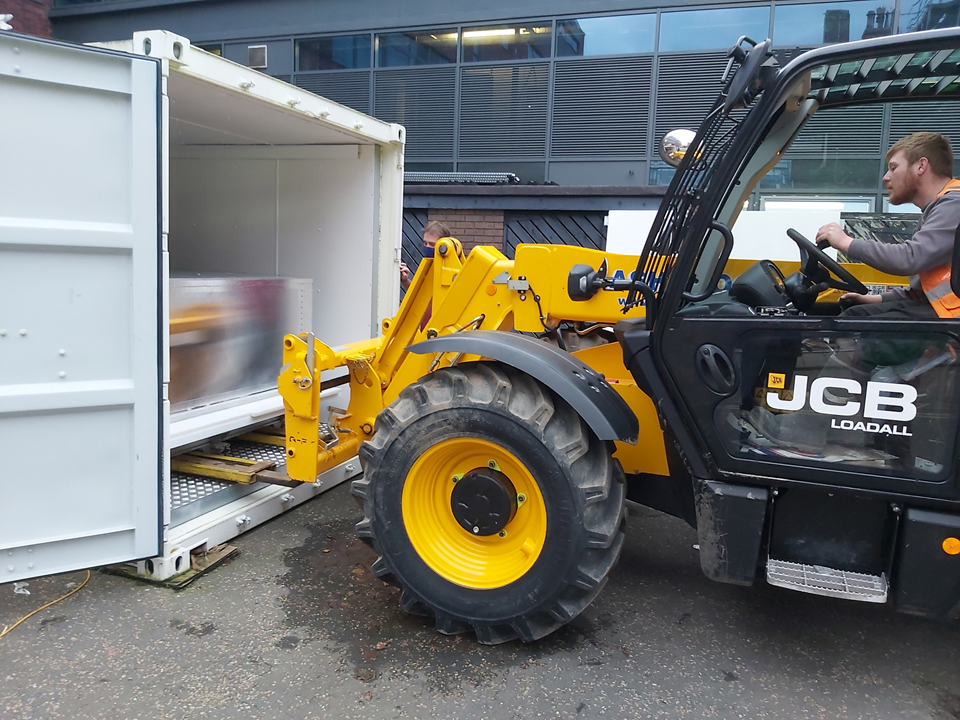
\includegraphics[width=0.8\linewidth]{Chapter3/Figs/Raster/detCon039_PutIn2.png}
% \captionof{figure}{The new detector being placed in the new container. (The upgrade was only partially completed at this time)} 
% \label{fig:detCon039_PutIn2}
% \end{figure}

\begin{figure}[htbp]
\centering
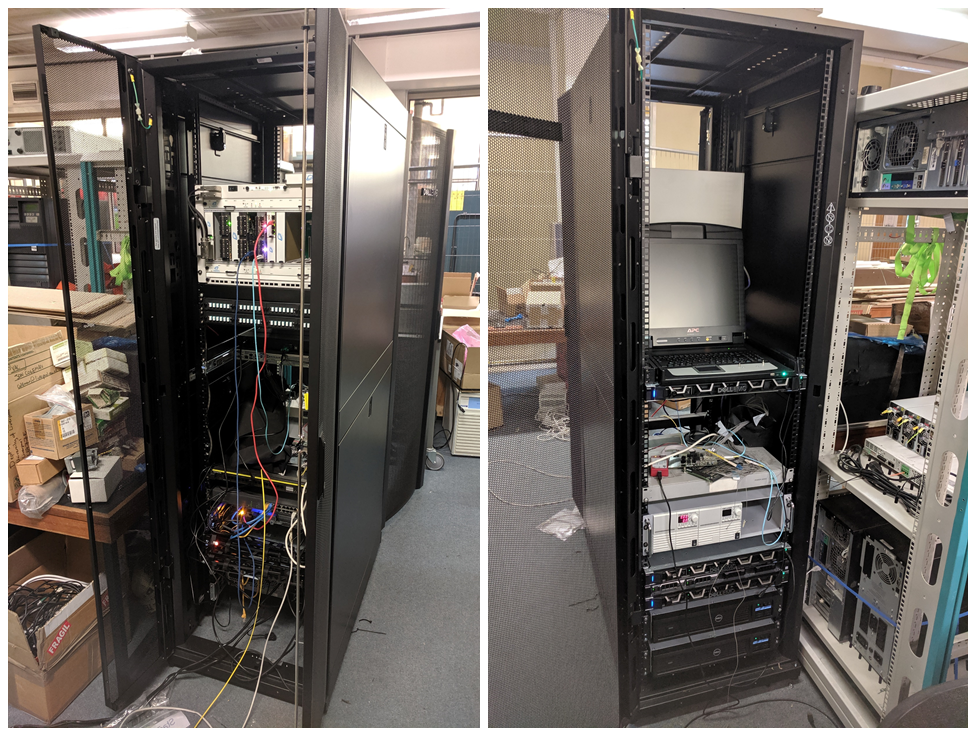
\includegraphics[width=0.7\linewidth]{Chapter3/Figs/Raster/detCon042b_Rack1.png}
\captionof{figure}{The computer rack for the upgraded detector from the back (left) and front (right).} 
\label{fig:detCon042b_Rack1}
\end{figure}

\begin{figure}[htbp]
\centering
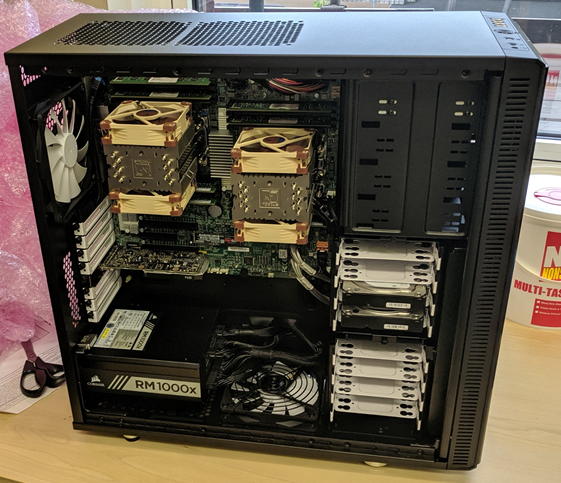
\includegraphics[width=0.8\linewidth]{Chapter3/Figs/Raster/detCon044_NewComputer.png}
\captionof{figure}{The new computer for the upgraded detector. It has two 32 core CPUs and 64\,Gb of Ram.} 
\label{fig:detCon044_NewComputer}
\end{figure}

% \begin{figure}[htbp]
% \centering
% 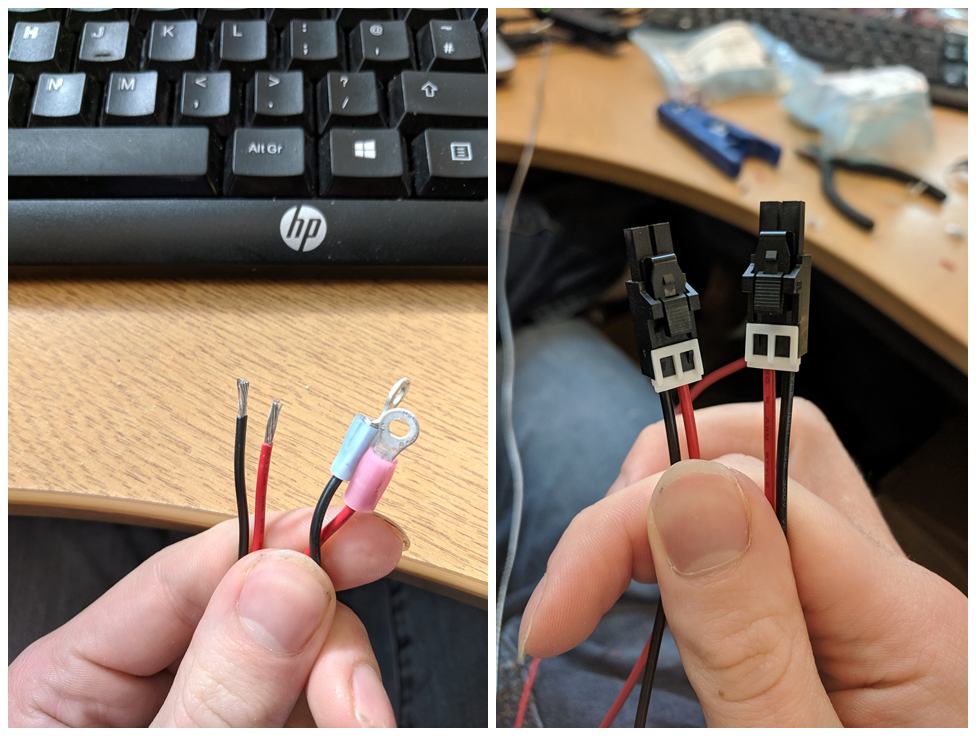
\includegraphics[width=0.7\linewidth]{Chapter3/Figs/Raster/detCon045b_PowerCabels1.png}
% \captionof{figure}{Power cables for the analogue boards that will attach to the central bus bars. \hl{may need to add some finer details remember to check with Carl}} 
% \label{fig:detCon045b_PowerCabels1}
% \end{figure}